\documentclass[%
reprint,
superscriptaddress,
%groupedaddress,
%unsortedaddress,
%runinaddress,
%frontmatterverbose,
%preprint,
showpacs,preprintnumbers,
%nofootinbib,
%nobibnotes,
%bibnotes,
 amsmath,amssymb,
 aps,
%pra,
%prb,
%prd,
prl,
%rmp,
%prstab,
%prstper,
%floatfix,
]{revtex4-1}

\usepackage{float}
\usepackage{graphicx}% Include figure files
\usepackage{dcolumn}% Align table columns on decimal point
\usepackage{bm}% bold math
\usepackage{bbold}
\usepackage{amssymb,amsmath}
\usepackage{hyperref}% add hypertext capabilities
%\usepackage[mathlines]{lineno}% Enable numbering of text and display math
%\linenumbers\relax % Commence numbering lines

%\usepackage[showframe,%Uncomment any one of the following lines to test
%%scale=0.7, marginratio={1:1, 2:3}, ignoreall,% default settings
%%text={7in,10in},centering,
%%margin=1.5in,
%%total={6.5in,8.75in}, top=1.2in, left=0.9in, includefoot,
%%height=10in,a5paper,hmargin={3cm,0.8in},
%]{geometry}



\usepackage{color}
\usepackage{amsfonts}
\usepackage{subfigure}
\usepackage{array}


\newcommand{\Tr}{\ensuremath{\operatorname{Tr}}}
\newcommand{\tr}{\ensuremath{\operatorname{tr}}}
\newcommand{\Omegaqq}{\ensuremath{\Omega_{\bar{q}q}}}
\newcommand{\vev}[1]{\ensuremath{\left\langle #1 \right\rangle}}
\newcommand{\einh}[1]{\ensuremath{\,\text{#1}}}
\newcolumntype{L}{>{\centering\arraybackslash}m{3cm}}



\newcommand{\overbar}[1]{\mkern 1.5mu\overline{\mkern-1.5mu#1\mkern-1.5mu}\mkern 1.5mu}

\definecolor{bjcol}{rgb}{1,.44,0.13}

% color def's

\definecolor{blue}{rgb}{0,0,1}
\newcommand{\colb}[1]{{\color{blue} #1}}
\definecolor{green}{rgb}{0,1,0}
\newcommand{\colg}[1]{{\color{green} #1}}
\definecolor{red}{rgb}{1,0,0}
\newcommand{\colr}[1]{{\color{red} #1}}
\newcommand{\colJ}[1]{{\color{cyan} #1}}
\definecolor{gray}{rgb}{.5,.5,.5}
\newcommand{\drop}[1]{{\sout{ {\color{gray} #1}}}}
\definecolor{darkgreen}{rgb}{.0,.5,.0}
\newcommand{\colL}[1]{{\color{darkgreen} #1}}


\def\Fig#1{Fig.~\ref{#1}} \def\Tab#1{Tab.~\ref{#1}}
\def\Figs#1{Figs.~\ref{#1}} \def\Tab#1{Tab.~\ref{#1}}
\def\Eqs#1{Eqs.~(\ref{#1})}
\def\Eq#1{Eq.~(\ref{#1})}
\def\eq#1{(\ref{#1})}
\def\eqref#1{(\ref{#1})}
\def\fig#1{Fig.~\ref{#1}}
\def\tab#1{Tab.~\ref{#1}}
\def\eqs#1{(\ref{#1})}
\def\Eqs#1{(\ref{#1})}
\def\sec#1{Sec.~\ref{#1}}
\def\app#1{Appendix~\ref{#1}}
\newcommand{\Phibar}{\ensuremath{\bar{\Phi}}}
\newcommand{\LPQM}{\ensuremath{\mathcal{L}_{\textrm{PQM}}}\xspace}

\def\dbar{{\mathchar'26\mkern-12mu d}}
\def\lA0{{\langle A_0 \rangle}}
\def\bA0{{\bar{A}_0}}
\def\lLA{{\langle L[A_0] \rangle}}
\def\lL{{\langle L \rangle}}
\def\lLc{{\langle L^\dagger \rangle}}
\def\lLAc{{\langle L^\dagger[A_0] \rangle}}


\def\dr{{D\!\llap{/}}\,}
\def\Dr{{D\!\llap{/}}\,}
\def\ipv{\vec{p}\llap{/}}
\def\pslash{p\llap{/}}

\def\0#1#2{\frac{#1}{#2}}

\newcommand{\bsig}{\ensuremath{\bar{\sigma}}}
\newcommand{\lsm}{L\ensuremath{\sigma}M\xspace}
\newcommand{\pT}{\ensuremath{T_0}}
\newcommand{\Tl}{\ensuremath{T_\chi}}
\newcommand{\Ts}{\ensuremath{T_\chi^s}}
\newcommand{\Tchi}{\ensuremath{T_\chi}}
\newcommand{\Td}{\ensuremath{T_d}}
\newcommand{\Tc}{\ensuremath{T_c}}
\newcommand{\muc}{\ensuremath{\mu_c}}
\newcommand{\coloronl}{(color online)\xspace}

\newcommand{\mrm}[1]{\mathrm{#1}}
\def\qbar{\bar{q}}
\newcommand{\sx}{\sigma_{x}}
\newcommand{\sy}{\sigma_{y}}

%%%%%%%%%%%%%% for corrections %%%%%%%%%%%
\newcommand{\colsy}[1]{\textcolor{blue}{#1}}
\newcommand{\colrw}[1]{\textcolor{cyan}{#1}}
\newcommand{\colwjf}[1]{\textcolor{red}{#1}}

%
%%%%%%%%%%%%%%%%%%%%%%%%%%%%%%%%%%%%%%%%%%%%%%%%%%%%%%%%%%%%%%%%%%%%%%%%%%%%%

\graphicspath{{./figures/}{./}}

\begin{document}

\preprint{}

\title{An estimate for the location of QCD critical end point
}

\author{Shi Yin}
\affiliation{School of Physics, Dalian University of Technology, Dalian, 116024,
  P.R. China}

\author{Rui Wen}
\affiliation{School of Physics, Dalian University of Technology, Dalian, 116024,
  P.R. China}

\author{Wei-jie Fu}
\email{wjfu@dlut.edu.cn}
\affiliation{School of Physics, Dalian University of Technology, Dalian, 116024,
  P.R. China}

%\date{\today}% It is always \today, today,
             %  but any date may be explicitly specified

\begin{abstract}
We investigate the relationship between the peak value of baryon number fluctuation kurtosis and the critical baryon chemical potential. At the same time, the freeze-out curves under different location of the critical end point. We control the location of the critical end point by a new cutoff scale which can remove the fermion vacuum fluctuation from the flow equations. We believe the relation between the kurtosis peak value and the chemical potential of critical end point (CEP) can give us a new way to predict the location of the CEP. This work is done under the low energy Polyakov-quark-meson (PQM) model with the functional renormalization group (FRG) approach.
\end{abstract}
%\pacs{Valid PACS appear here}% PACS, the Physics and Astronomy
\pacs{11.30.Rd, %Chiral symmetries
         11.10.Wx, %Finite-temperature field theory
         05.10.Cc, %Renormalization group methods
         12.38.Mh  %Quark-gluon plasma
     }                             % Classification Scheme.
%\keywords{Suggested keywords}%Use showkeys class option if keyword
                              %display desired
\maketitle
%\tableofcontents
%%%%%%%%%%%%%%%%%%%%%%%%%%%%%%%%%%%%%%%%%%%%%%%%%%%%%%%%%%%
%%%%%%%%%%%%%%%%%%%%%%%%%%%%%%%%%%%%%%%%%%%%%%%%%%%%%%%%%%%
\paragraph*{Introduction ---\!\!\!}
\label{sec:int}
The nature of the elementary particle has attracted the research interest of countless scientists. In the last century, hadrons are found to consist of quark gluons with the strong interaction. The Quantum Chromodynamics (QCD) is the most successful theory for describing strong interactions. Then people found a lot of marvellous properties of the quark. In the past decades, the deconfinement phase transition of the quark is a hot research direction. The particle accelerators around the world have experiments on the research of the QCD phase structure of the phase diagram. The low density area of the phase diagram is well studied, however, the physical property at high baryon chemical potential, i.e., the high density area is hard to investigate. In the experimental field, the Relativistic Heavy Ion Collider (RHIC) that provides us with a lot of experimental data at the high density part, see \cite{Adamczyk:2013dal,Luo:2015ewa,Luo:2017faz}. In the 

\par
This paper has been divided into three parts. Firstly, we give a simple discuss of the baryon number fluctuation and the relationship between the fermion vacuum fluctuation and the location of the CEP. Secondly, the theoretical framework of the FRG as well as the Polyakov-quark-meson model are introduced. At the same time, the method we use to cutoff the fermion vacuum fluctuation is also discussed. Finally, we give our numarical results and the comparison of the lattice results, then end with a summary.

%%%%%%%%%%%%%%%%%%%%%%%%%%%%%%%%%%%%%%%%%%%%%%%%%%%%%%%%%%%%%
%%%%%%%%%%%%%%%%%%%%%%%%%%%%%%%%%%%%%%%%%%%%%%%%%%%%%%%%%%%%%
\paragraph*{Baryon number fluctuations and the fermion vacuum fluctuation ---\!\!\!}
\label{sec:EoS}
The kurtosis of the baryon number fluctuation is the core of our work, for the significant role it plays in the experiment area of the QCD phase structure. The calculation of the baryon number fluctuation can be done using the following formula, 
\begin{align}
   \chi_n^{B}&=\frac{\partial^n}{\partial (\mu_B/T)^n}\frac{p}{T^4}\,,\label{eq:suscept}
\end{align}
in which the $\mu_B=3\mu$ is the beryon chemical potential that is triple of the quark chemical potential. Then we can obtain the first to fourth order of the beryon number fluctuation known as the generalized susceptibilities,
\begin{align}
  \chi_2^B&=\frac{1}{VT^3}\langle(\delta N_B)^2\rangle\,,\\[2ex]
  \chi_4^B&=\frac{1}{VT^3}\Big(\langle(\delta N_B)^4\rangle-3\langle(\delta N_B)^2\rangle^2\Big)\,,
\end{align}
The meaning of the angle brackets stands for the average value, and the $\delta N_B$ stands for the difference between the $N_B$ and $\langle N_B\rangle$ which reads $\delta N_B:=N_B - \langle N_B\rangle$.\par For the purpose of comparing our calculation with the experimental and lattice results, we divide the fourth and second order of the baryon number fluctuations to get the kurtosis which is the observable in the experiments, e.g., $\kappa\sigma^2=\chi^B_4/\chi^B_2$. More details discussion about baryon number fluctuation see e.g., \cite{Fu:2015naa}. Here we investigate the relationship of the maximum value of the kurtosis and the fermion vacuum fluctuation.
\par We find that the location of the critical end point would change with different fermion vacuum contribution we involve in our calculation. In this work we add a new cutoff scale into the functional renormalisation group flow equation to restrict the fermion vacuum fluctuation and study the behavior of the location of the critical end point under the different cutoff. From the previous work of the low energy effective theory under the FRG, the flow equation of the effective potential contain the full contribution of the fermion vacuum part throughout the integral interval which is cover from the infrared point to the ultraviolet point. The effect of the fermion vacuum contribution is studied in the mean field approximation, see \cite{Skokov:2010sf}. We can tell that the fermion vacuum fluctuation can suppress the baryon number fluctuation at finite temperature and density. If the new cutoff scale get the value of the UV scale, the flow return to the previous which includes all the fermion vacuum term. If the cutoff scale get the value of the IR scale, the flow get the result of the mean-field approximation. The neglect of the fermion vacuum part is known as the no-sea approximation.
%%%%%%%%%%%%%%%%%%%%%%%%%%%%%%%%%%%%%%%%%%%%%%%%%%%%%%%%%%%%%
%%%%%%%%%%%%%%%%%%%%%%%%%%%%%%%%%%%%%%%%%%%%%%%%%%%%%%%%%%%%%
\paragraph*{Polyakov-Quark-meson model and the cutoff ---\!\!\!}
\label{sec:pqm}
This work is done under the two quark flavor Polyakov-quark-meson model with functional renormalisation group approach. We give the infrared cutoff scale dependent effective action
\begin{align}
  \Gamma_k=&\int_x \bigg\{Z_{q,k}\bar{q} \Big [\gamma_\mu \partial_\mu -\gamma_0(\hat\mu+igA_0) \Big ]q \nonumber\\[2ex]
  &+\frac{1}{2}Z_{\phi,k}(\partial_\mu \phi)^2\nonumber+h_k\bar{q}\big(T^0\sigma+i\gamma_5\vec{T}\cdot \vec{\pi}\big)q\\[2ex]
  &+V_k(\rho)-c\sigma \bigg\}\,,
\label{eaction}
\end{align}
with the 4 dimension integral $\int_x=\int^{1/T}_0dx_0\int d^3x$. The $k$ is the FRG infrared (IR) cutoff scale which is running from the ultraviolet (UV) scale to 0. The meson field is defined as $\phi=(\sigma,\vec{\pi})$, and $\rho=\phi^2/2$. $\vec{T}$ is the generators of the $SU(N_f)$ group here we have $N_f=2$. The generators satisfy $\mathrm{Tr}(T^iT^j)=\frac{1}{2}\delta^{ij}$, $T^0=\frac{1}{\sqrt{2N_f}}\mathbb{1}_{N_f\times N_f}$. The $-c\sigma$ gives the chiral symmetry breaking in our theory. In this work we get the results under the local potential approximation (LPA), under which $\partial_tZ_{\phi,q}=0$, $\partial_t h_k=0$. The $t$ is RG time with $t=\mathrm{ln}(k/\Lambda)$. We choose the UV cutoff scale $\Lambda$ to 700$\mathrm{MeV}$. The effective potential $V_k(\rho)$ involves the infermation of the meson chiral symmetry breaking. Here we solve the flow equation of the effective potential by the Taylor expansion around the expansion point $\kappa$. The expansed meson potential is $V_k(\rho)=\sum^{N_v}_{n=0}\frac{\lambda_{n,k}}{n!}(\rho-\kappa_k)^n$. In this work, we choose $N_v=5$ for the good convergence of the fix expansion point $\partial_t\kappa_k=0$. In order to get the pressure, the thermodynamical potential should be calculated. The definition of the thermodynamical potential is $\Omega[T,\mu]=V_{k=0}(\rho)+V_{glue}(L,\bar{L})-c\sigma$. The glue potential is a function of the traced Polyakov loop $L$ and the complex conjugate $\bar{L}$. They are in concerning with the gluonic background field $A_0$ by $L=\frac{1}{N_c}\langle \mathrm{Tr}\mathcal{P}\rangle$, $\bar{L}=\frac{1}{N_c}\langle \mathrm{Tr}\mathcal{P}^\dagger\rangle$ with $\mathcal{P}=\mathcal{P}\mathrm{exp}\big(ig\int^\beta_0d\tau A_0(\tau)\big)$. Then the pressure of the system can be computed by the thermodynamical potential $p=-\Omega[T,\mu]$.\par To obtain the CEP location of our system under different cutoff scale $\Lambda_2$, we use the Pion decay constant as the criterion. The Pion decay constant is the order parameter of the phase transition, given by $f_{\pi}=\langle \sigma\rangle$. The peak value of $\partial f_\pi/\partial T$ is used to determine the crossover line at low baryon chemical potential. When a relatively large difference of the $f_\pi$ appear appear between two adjacent temperatures, we believe the crossover is already convert to the first order phase transition. The temperature and baryon chemical potential between these two kinds of phase transition fix the location of the CEP.\par We can derive the flow equation by the Wetterich equation see \cite{Wetterich:1992yh}, reads
\begin{align}
\partial_t \Gamma_k[\Phi]=\frac{1}{2}\mathrm{Tr}\big(G_{\phi\phi,k}\partial_t R^\phi_k\big)-\mathrm{Tr}\big(G_{q\bar{q},k}\partial_t R^q_k\big).
\label{weq}
\end{align}
 In the LPA situation, we focus on the flow of effective potential. Take the effective potential $V_k(\rho)$ in the effective action Eq. (\ref{eaction}) into Eq. (\ref{weq}). Then flow equation can be derived
\begin{align}
\begin{split}
   \partial_t V_k(\rho)=&\frac{k^4}{4\pi^2}\big[(N^2_f-1)l^{B,4}_{0}(\bar{m}^2_{\pi,k},\eta_{\phi,k};T)\\
   &+l^{(B,4)}_{0}(\bar{m}^2_{\sigma,k},\eta_{\phi,k};T)\\
   &-4N_cN_fl^{(F,4)}_{0}(\bar{m}^2_{q,k},\eta_{q,k};T,\mu)\big].
\end{split}
\end{align}
\par The anomalous dimensions of the fermion and boson is all 0 here. The $l^{(F,4)}_{0}$ in the flow equation stands for the fermion threshold function. The analytical form of the threshold function is 
\begin{align}
\begin{split}
l^{(F,d)}_{0}&(\bar{m}^2_{q,k},\eta_{q,k};T,\mu)=\frac{1}{z_q(d-1)\sqrt{1+\bar{m}^2_{q,k}}}(1-\frac{\eta_{q,k}}{d})\\
&\times(1-n_F(\bar{m}^2_{q,k},z_q;T,\mu)-n_F(\bar{m}^2_{q,k},z_q;T,\mu))
\end{split}
\end{align}
which contains all contribution of the fermion vacumm fluctuation. We take place this with another threshold function with no fermion vacuum part 
\begin{align}
\begin{split}
j^{(F,d)}_{0}&(\bar{m}^2_{q,k},\eta_{q,k};T,\mu)=\frac{1}{z_q(d-1)\sqrt{1+\bar{m}^2_{q,k}}}(1-\frac{\eta_{q,k}}{d})\\
&\times(-n_F(\bar{m}^2_{q,k},z_q;T,\mu)-n_F(\bar{m}^2_{q,k},z_q;T,\mu))
\end{split}
\end{align}
\par Then we devided the integral of the flow equation into two parts by the new cutoff scale $\Lambda_2$ between the IR and UV scales. The integral between the IR scale and $\Lambda_2$ is the flow equation with the fermion vacuum contribution the other side of the integral that between the $\Lambda_2$ and UV scale is the flow equation without the fermion vacuum contribution. Now we can control the quantity of the fermion vacuum part by changing the new cutoff $\Lambda_2$.
%%%%%%%%%%%%%%%%%%%%%%%%%%%%%%%%%%%%%%%%%%%%%%%%%%%%%%%%%%%%%
%%%%%%%%%%%%%%%%%%%%%%%%%%%%%%%%%%%%%%%%%%%%%%%%%%%%%%%%%%%%%
\paragraph*{Results and Summary ---\!\!\!}
\label{sec:res}
We will give some numarical results and summarize the outcome in the last section. As mentioned in the previous section, we add a new cutoff scale to remove part of the fermion vacuum contribution from solving our FRG effective potential flow equation. Then we calculate the two and four order generalized susceptibilities and their ratio which is the kurtosis. The location of the CEP is also obtained by the $f_\pi$ under several baryon chemical potential. \par The Tab. \ref{tab:cut} gives the relationship between the new cutoff scale and the location of the CEP. We can easily tell from the table, with the decrease of the $\Lambda_2$ the baryon chemical potential of the CEP  b gradually gets low and the temperature of the CEP increases. In other words, the CEP is moving towards the left upper corner of the QCD phase diagram. When the cutoff comes to zero, i.e., the no-sea approximation, the CEP even reached $\mu_B=335\,\,\mathrm{MeV}$ that is a vary small value. It is clear, there is a significant correlation between the CEP location and the fermion vacuum fluctuation. From these number we can easily see that the change of the CEP is bigger at the middle value of the cutoff, from 100 MeV to 500 MeV.\par In addition to affecting the location of the CEP, it also affects the kurtosis of the baryon number fluctuation. We know that the kurtosis as a function of temperature under the mean-field approximation has a peak. If the fermion vacuum fluctuation is included, the peak will be surpress and come to the value 1 see, e.g., \cite{Skokov:2010sf}. So we give a diagram that show us the dependence of the kurtosis peak value on the baryon chemical potential of CEP. Because the CEP chemical potential is related to the cutoff scale $\Lambda_2$, the diagram can also be understood as the relation between the kurtosis peak value and the cutoff scale $\Lambda_2$. The picture is clear, with the increase of the CEP chemical potential the kurtosis peak value has undergone a gradual slowing down process. In the end, it come to 1. This relationship suggest that maybe we can use the peak value of the kurtosis to predict the location of the CEP, especially in the lattice QCD simulation.  As we all know, the sign problem limits the computation to the small baryon chemical potential area, e.g., $\mu_B/T\leqslant 3$. So we put the lattice results in our picture for comparison. We put the results of the HotQCD Collaboration \cite{Bazavov:2017dus,Bazavov:2017tot} and the Wuppertal-Budapest Collaboration \cite{Borsanyi:2013hza}. Here we choose the data of which have the maximum upper bound of the error bar. The results in Fig. \ref{fig:cp} is clear, the intersection of our curve and the lattice results is at around $\mu_B=700$ MeV. \par Now we give a shirt summary of this paper. In this work, we study the relation of the fermion vacuum fluctuation and the CEP location of the QCD phase diagram under the functional renormalisation group. The results are performed in the two flavor PQM model. It is found that the kurtosis peak value has a obviously dependent on the cutoff of the fermion vacuum part. The lattice results are compared in the Fig. \ref{fig:cp} and they are intersection at about $\mu_B=700$ MeV of the CEP. We may not be able to jump to conclusions that the CEP of the lattice simulation is around the $\mu_B=700$ MeV, because our calculation is just accomplished under the LPA truncation. In the future, further work is required to add the full truncation into the calculation and more careful analysis is needed to study thoroughly of this relation.
%
%%%%%%%%%%%%%%%%%%%%%%%%%%%%%
\begin{figure}[t]
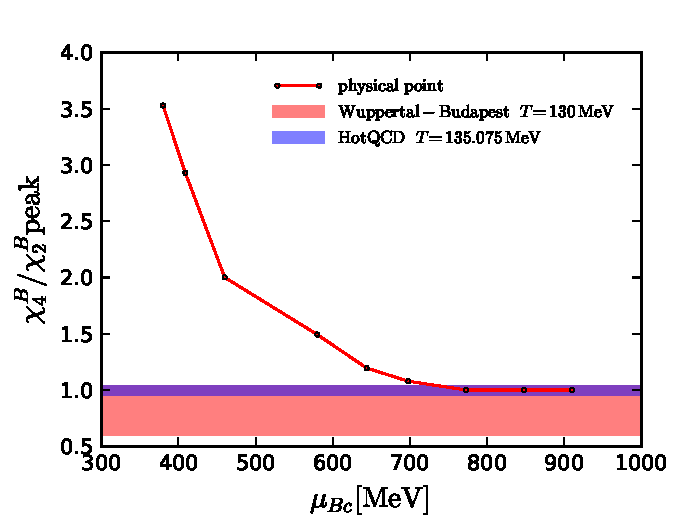
\includegraphics[width=0.5\textwidth]{cp}
\caption{The relation between the maximum baryon number fluctuation kurtosis value under $\mu_B=0$ and the baryon chemical potential of the critical end point. The lattice data comes from the \cite{Bazavov:2017dus,Bazavov:2017tot} which are the results of HotQCD Collaboration and \cite{Borsanyi:2013hza} by Wuppertal-Budapest Collaboration}\label{fig:cp}
\end{figure}
%%%%%%%%%%%%%%%%%%%%%%%%%%%%%
%
%
 %%%%%%%%%%%
\begin{table}[t]
  \centering
  \begin{tabular}{c||c|c|c|c|c|c|c|c}
    \hline
    $\Lambda_2\,\,(\mathrm{MeV})$ & 0 & 100 & 200 & 300 & 400 & 500 & 600 & 700  \rule{0pt}{2.6ex}
\rule[-1.2ex]{0pt}{0pt}\\ \hline\hline
    $T_c\,\,(\mathrm{MeV})$ &124& 123 & 117 &110 &98&97&95&89 \\\hline
    $\mu_Bc\,\,(\mathrm{MeV})$ &335 &345 &435 &552&655&725&770&785\\\hline

  \end{tabular}
  \caption{The location of the critical point and the corresponding value of the cutoff $\Lambda_2$.} 
  \label{tab:cut}
\end{table}

%%%%%%%%%%%%%%%%%%%%%%%%%%%%%%%%%%%%%%%%%%%%%%%%%%%%%%%%%%%

\begin{acknowledgments}

\vspace{0.1cm} {\it Acknowledgments -} We thank the members of the fQCD collaboration \cite{fQCD} for work on related projects. The work was supported by the National Natural Science Foundation of China under Contracts Nos. 11775041.

\end{acknowledgments}

%%%%%%%%%%%%%%%%%%%%%%%%%%%%%%%%%%%%%%%%%%%%%%%%%%%%%%%%%%%%%
%%%%%%%%%%%%%%%%%%%%%%%%%%%%%%%%%%%%%%%%%%%%%%%%%%%%%%%%%%%%%

% The \nocite command causes all entries in a bibliography to be
% printed out whether or not they are actually referenced in the
% text. This is appropriate for the sample file to show the different
% styles of references, but authors most likely will not want to use
% it.  \nocite{*}

%\bibliography{refspec}% Produces the bibliography via BibTeX.
\bibliography{ref-lib}% Produces the bibliography via BibTeX.


\end{document}
